\section{Séquencement}
	\label{sec:sequencement}
	Pour établir notre planification, nous avons utilisé le logiciel MS Project. Les diagrammes ci-dessous tiennent compte des différents jalons qui ont été posés, soit imposés à tous dans les projets de 4INFO, soit définis nous-même.

	\subsection{Diagramme de Gantt}
		Le diagramme de Gantt visible sur la \ffigure{} \ref{fig:gantt} illustre le séquencement de notre projet. Les tâches ont été attribuées à une personne, et les durées ont été calculées pour une moyenne d'une heure-et-demi de travail personnel par jour. Les semaines du 18 et 25 mai, bloquées pour les 4INFO, la durée du travail personnel a été porté à 4h par jour. Dans le cas des tâches réalisées par plusieurs personnes, les contributions de ces différentes personnes sont séparées par des pointillés.  
	
	\subsection{Répartition de la charge de travail}
		Le planning de la \ffigure{} \ref{fig:planning_charge} illustre la répartition par personnes du temps de réalisation des taches ainsi que le cumul des heures de travail pour chacun. Nous avons essayé d'être autant que possible homogènes dans la répartition du temps de travail, les différences de répartition étant la conséquence de l'irrégularité de durée des taches.

	\subsection{Utilisation des ressources}
		Le dernier graphique à la \ffigure{} \ref{fig:taux_utilisation} rend compte de l'utilisation du temps de travail pour l'ensemble du groupe, que nous avons fixé à raison de une heure trente par jour en semaine normale. On distingue facilement les trois versions grâce au taux de charge de travail.  

		\begin{landscape}
		 	\begin{figure}
	            \centering
	            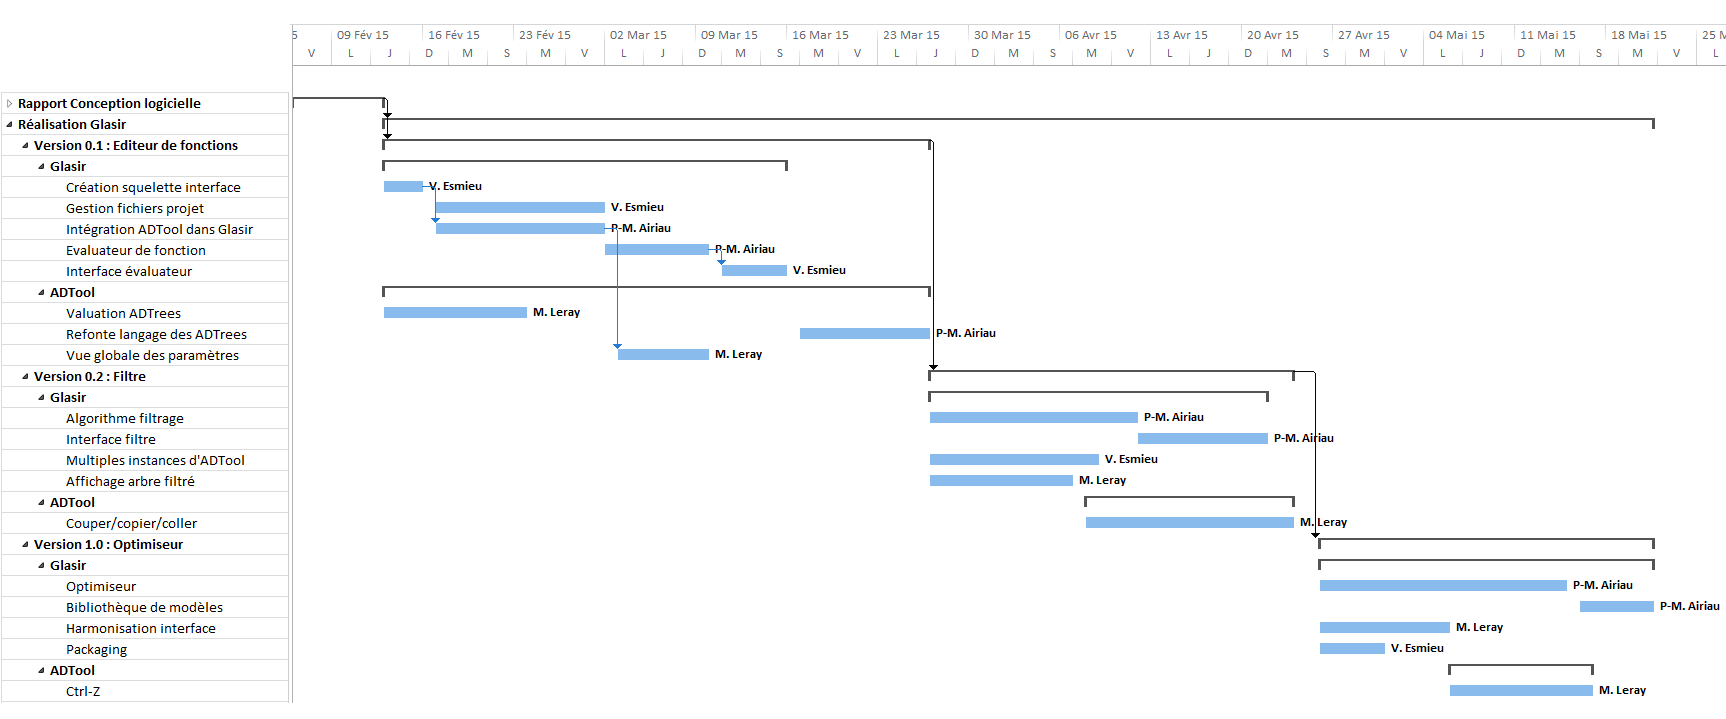
\includegraphics[height=0.70\textwidth]{figure/DiagGantt.png}
	            \caption{Diagramme de Gantt présentant la chronologie des tâches.}
	            \label{fig:gantt}
	        \end{figure}
	    \end{landscape}

		\begin{landscape}
		 	\begin{figure}
	            \centering
	            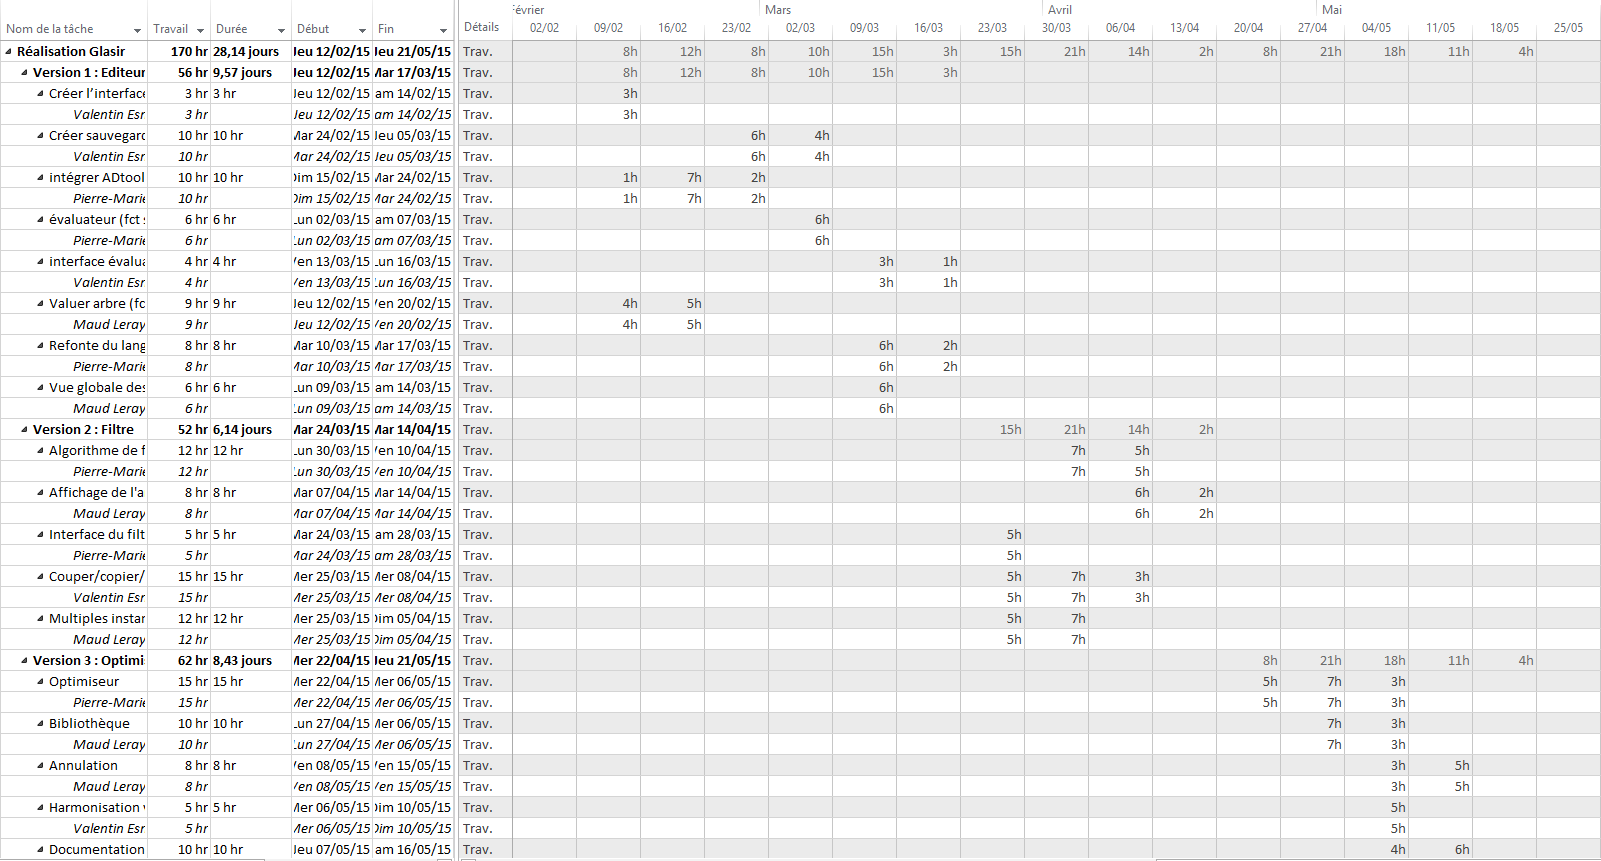
\includegraphics[height=0.70\textwidth]{figure/RepartitionTaches2.png}
	            \caption{Planning des charges réparties par personne}
	            \label{fig:planning_charge}
	        \end{figure}
	    \end{landscape}

		\begin{landscape}
		 	\begin{figure}
	            \centering
	            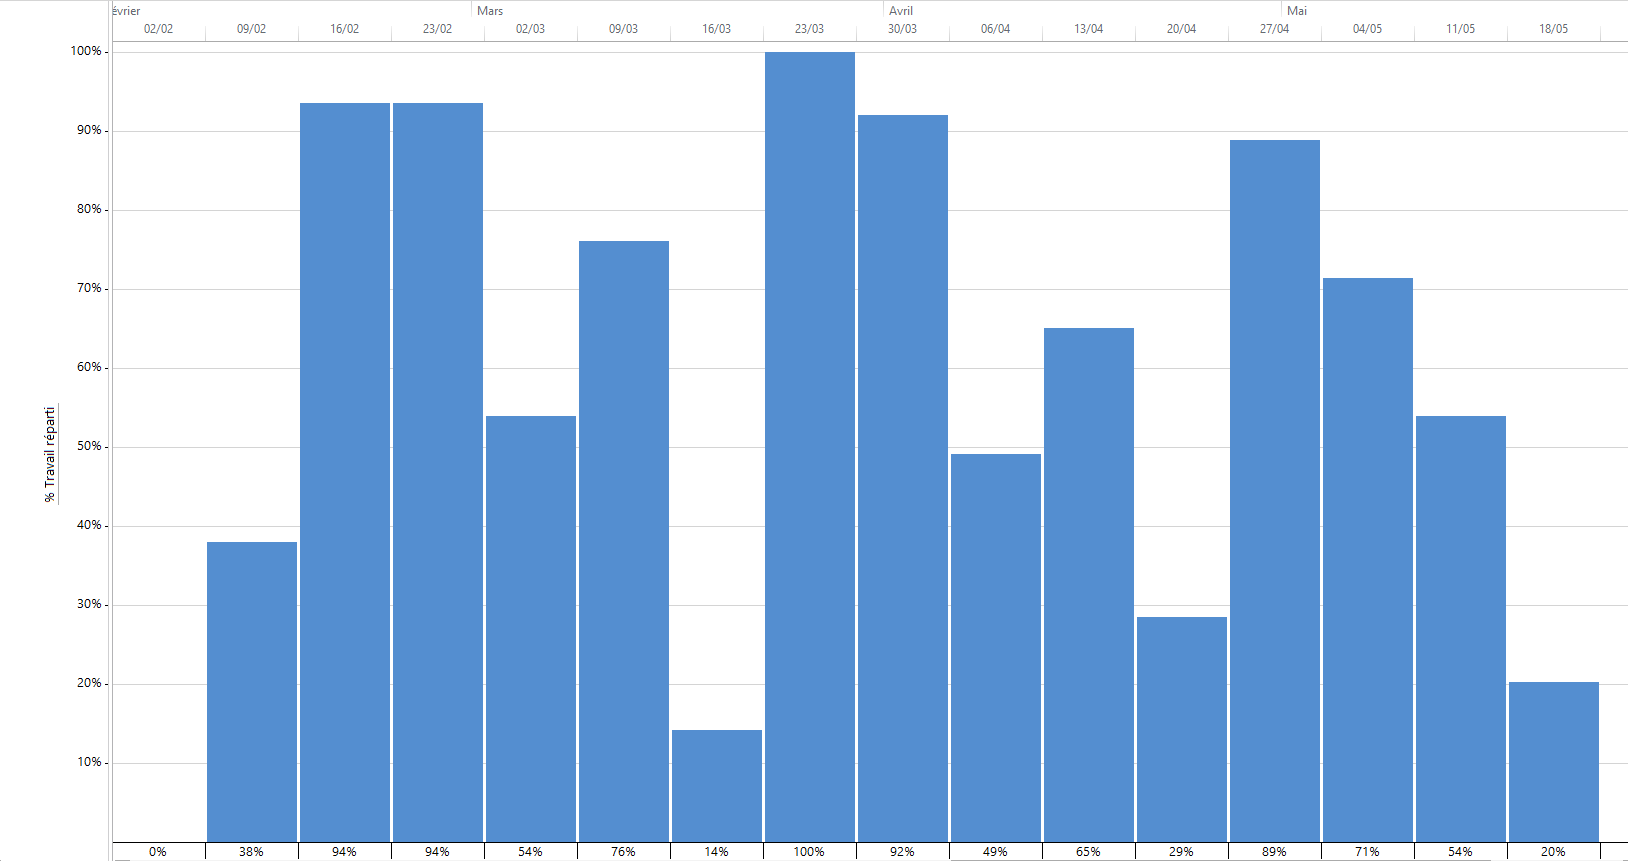
\includegraphics[height=0.70\textwidth]{figure/TauxUtilisation.png}
	            \caption{Taux d'utilisation du temps de travail de l'ensemble du groupe }
	            \label{fig:taux_utilisation}
	        \end{figure}
	    \end{landscape}